\ylDisplay{Vaakumkahur} % Ülesande nimi
{Andreas Valdmann} % Autor
{lahtine} % Voor
{2014} % Aasta
{G 2} % Ülesande nr.
{2} % Raskustase
{
% Teema: Dünaamika
\ifStatement
Joonisel on kujutatud niinimetatud vaakumkahur. Laadimiseks pistetakse laskemoonaks olev pall vaakumkahuri toru vasakpoolsest otsast sisse. Seejärel kaetakse toru mõlemad otsad kergestirebeneva õhukindla membraaniga, näiteks fooliumiga, ning pumbatakse torust õhk välja. Nüüd on vaakumkahur laskevalmis. Tulistamiseks purustatakse vasakpoolne membraan, mille tagajärjel hakkab pall toru parempoolse otsa poole sööstma. Piisavalt pika toru korral purustab pall parempoolse membraani ning lendab torust välja. Olgu palli läbimõõt võrdne toru siseläbimõõduga $d=\SI{4,0}{cm}$, palli mass $m=\SI{24}{g}$ ja asugu pall enne tulistamist $l=\SI{150}{cm}$ kaugusel toru parempoolsest otsast. Kui suur on palli kiirus vahetult enne parempoolse membraani läbimist? Õhurõhk on $P_0=\SI{100}{kPa}$. Hõõrdumisega pole tarvis arvestada.
\begin{center}
 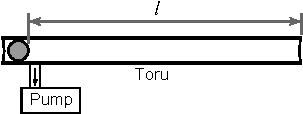
\includegraphics[width=0.75\textwidth]{2014-lahg-02-vaakumkahur.pdf}
\end{center}
\fi


\ifHint
Pall jaotab kahuritoru kaheks kambriks. Pärast vasakpoolse membraani purustamist hakkab vasakpoolses kambris olev gaas palli paremale poole suruma.
\fi


\ifSolution
Pall jaotab kahuritoru kaheks kambriks. Enne tulistamist on mõlemas kambris rõhk võrdne nulliga. Vasakpoolse membraani purustamisel täitub vasak pool torust välisõhuga ning palli poolte vahel tekib rõhkude vahe $\Delta P=P_0-0=P_0$. Pallile hakkab mõjuma jõud, mis on võrdne palli ristlõikepindala ja rõhkude vahe korrutisega: $F=P_0\pi d^2/4$. Newtoni 2. seaduse abil saame leida palli kiirenduse $a=F/m$. Ühtlaselt kiireneva liikumise korral kehtib seos
\[ l=\frac{v^2-v_0^2}{2a}, \]
kus $l$ on läbitud vahemaa ning $v_0$ ja $v$ on vastavalt alg- ja lõppkiirus. Kuna palli algkiirus on võrdne nulliga ning tahame leida lõppkiirust, siis avaldame
\[ v=\sqrt{2la}=\sqrt{\frac{2lP_0\pi d^2}{4m}}=d\sqrt{\frac{lP_0\pi}{2m}}.\]
Kasutades ülesandes antud arvväärtusi, saame palli kiiruseks vahetult enne parempoolse membraani läbimist $v=\SI{130}{m/s}$. Membraani purustamiseks kulub energiat ning seetõttu on palli väljumiskiirus sellest veidi väiksem, kuid võite isegi ette kujutada, et õhuke fooliumileht ei takista \SI{470}{km/h} kihutava palli lendu just märkimisväärselt.
\fi


\ifEngStatement
% Problem name: Vacuum cannon
Pictured below is a so-called vacuum cannon. To load it, a ball meant for ammunition is put into the left end of the vacuum cannon. Next, both ends of the tube are covered with an easily rupturing airproof membrane, for example foil, and then the air is pumped out of the tube. The vacuum cannon is now ready for firing. For firing, the membrane on the left is intentionally ruptured. As a result the ball starts to charge towards the right end of the tube. If the tube is long enough the ball ruptures the membrane on the right end and is fired out of the tube. Let us say that the diameter of the ball is equal to the inner diameter of the tube $d=\SI{4,0}{cm}$, the ball’s mass is $m=\SI{24}{g}$ and before the firing the ball is positioned at a distance $l=\SI{150}{cm}$ from the right end of the tube. What is the speed of the ball directly before rupturing the membrane on the right? Air pressure is $P_0=\SI{100}{kPa}$. Do not account for friction.
\begin{center}
  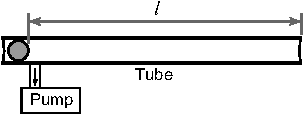
\includegraphics[width=0.75\textwidth]{2014-lahg-02-vaakumkahur_ing}
\end{center}
\fi


\ifEngHint
The ball divides the cannon tube into two chambers. After rupturing the left membrane the gas in the left chamber starts to press the ball to the right side.
\fi


\ifEngSolution
The ball divides the tube of the cannon into two chambers. Before firing the pressure in both chambers is equal to zero. By rupturing the membrane on the left the tube’s left side fills with outer air and between each side of the ball there is pressure difference $\Delta P=P_0-0=P_0$. The ball is starting to be affected by a force that is equal to the product of the ball’s cross-sectional area and the pressure difference: $F=P_0\pi d^2/4$. With the Newton’s second law we can find the ball’s acceleration $a=F/m$. During a uniformly accelerating motion the equation 
\[ l=\frac{v^2-v_0^2}{2a}, \] 
applies, where $l$ is the distance covered and $v_0$ and $v$ are respectively the initial and final speed. Since the initial speed of the ball is equal to zero and we want to find the final speed, we can express 
\[ v=\sqrt{2la}=\sqrt{\frac{2lP_0\pi d^2}{4m}}=d\sqrt{\frac{lP_0\pi}{2m}}.\] 
Using the primary data we find that the speed of the ball momentarily before going through the right membrane is $v=\SI{130}{m/s}$. It takes energy to rupture the membrane and therefore the exiting speed of the ball is slightly smaller but you can imagine yourself that a thin foil layer does not hamper the flight of a ball flying with speed 470 km/h.
\fi
}